\documentclass[twocolumn]{sagej}

% Load basic packages
\usepackage{balance}		% to better equalize the last page
\usepackage{graphics}		% for EPS, load graphicx instead
\usepackage{times}			% comment if you want LaTeX's default font
\usepackage{url}			% llt: nicely formatted URLs
\usepackage{dblfloatfix}	% allow placement of a page-width figure at top or bottom of page

% llt: Define a global style for URLs, rather that the default one
\makeatletter
\def\url@leostyle{%
  \@ifundefined{selectfont}{\def\UrlFont{\sf}}{\def\UrlFont{\small\bf\ttfamily}}}
\makeatother
\urlstyle{leo}

\usepackage{tikz}
% Make sure hyperref comes last of your loaded packages,
% to give it a fighting chance of not being over-written,
% since its job is to redefine many LaTeX commands.
\usepackage[pdftex]{hyperref}

\newcommand{\modelfraction}{0.65}
\newcommand{\betweenmodels}{0.8cm}
\newcommand{\plotfraction}{0.85}

% End of preamble. Here comes the document.
\begin{document}

\title{Performance analysis of a PDEVS simulator supporting multiple synchronization protocols}

\author{Ben Cardoen\affilnum{1}, Stijn Manhaeve\affilnum{1}, Yentl Van Tendeloo\affilnum{1}, and Jan Broeckhove\affilnum{1}}

\affiliation{\affilnum{1}University of Antwerp, Belgium}

\corrauth{Yentl Van Tendeloo\\
University of Antwerp\\
Middelheimlaan 1\\
2020 Antwerp, Belgium}

\email{Yentl.VanTendeloo@uantwerpen.be}

\begin{abstract}
With the ever increasing complexity of simulation models, parallel simulation becomes necessary to perform simulation within reasonable time bounds.
The built-in parallelism of Parallel DEVS is often insufficient to tackle this problem on its own.
Several synchronization protocols have been proposed, each with their distinct advantages and disadvantages.
Due to the significantly different implementation of these protocols, most Parallel DEVS simulation tools are limited to only one such protocol.
In this paper, we present a Parallel DEVS simulator, grafted on C++11 and based on PythonPDEVS, supporting both conservative and optimistic synchronization protocols.
The simulator not only supports both protocols but also has the capability to switch between them at runtime.
The simulator complements each of the synchronization protocols with the PDEVS protocol.
We evaluate the performance gain obtained by choosing the most appropriate synchronization protocol.
A comparison is made to adevs in terms of CPU time and memory usage, to show that our modularity does not hinder performance.
We compare the speedup obtained by synchronization with that of the inherent parallelism of PDEVS in isolation and combination, and contrast the results with the theoretical limits.
We further allow for an external component to gather simulation statistics, on which runtime switching between the different synchronization protocols can be based.
Model allocation is also studied to see how our conservative and optimistic synchronization protocols are affected by good and bad allocations.

\end{abstract}

\maketitle

\section{Introduction}
\label{sec:1-introduction}
\textsf{DEVS}~\cite{ClassicDEVS} is a popular formalism for modelling complex dynamic systems using a discrete-event abstraction.
In fact, it can serve as a simulation ``assembly language'' to which models in other formalisms can be mapped~\cite{DEVSbase}.
A number of tools have been constructed by academia and industry that allow the modelling and simulation of \textsf{DEVS} models.

But with the ever increasing complexity of simulation models, parallel simulation becomes necessary to perform the simulation within reasonable time bounds.
And while \textsf{Parallel DEVS}~\cite{ParallelDEVS} was introduced to increase parallelism, this is often insufficient.
Several synchronization protocols from the discrete event simulation community~\cite{FujimotoBook} have been applied to \textsf{DEVS} simulation.
While several parallel \textsf{DEVS} simulation kernels exist, they are often limited to a single synchronization protocol.
The reason for different synchronization protocols, however, is that their distinct nature makes them applicable in different situations, each outperforming the other in specific models.
The applicability of parallel simulation capabilities of current tools is therefore limited.

This paper introduces DEVS-Ex-Machina\footnote{\url{https://bitbucket.org/bcardoen/devs-ex-machina}} (``dxex''), our simulation tool which offers multiple synchronization protocols: no synchronization (sequential execution), conservative synchronization, or optimistic synchronization.
The selected synchronization protocol is transparent to the simulated model: users should merely determine, which protocol they wish to use.
Users who simulate a wide variety of models, with different ideal synchronization protocols, can simply run the same model with different synchronization protocols.
We investigate in this paper how model allocation and uncertainty determine the choice between synchronization protocols. 
The synchronization overhead is demonstrated by reducing the computational load of a model to near zero. 

Our tool is based on PythonPDEVS, but implemented in C++11 for increased performance, using features from the new C++14 standard when possible.
Unlike PythonPDEVS dxex only supports multicore parallelism.

We implemented a model that, depending on a single parameter, changes its ideal synchronization protocol. We demonstrate using several models the factors influencing the performance under a given synhronization protocol.
Dxex, then, is used to compare simulation using exactly the same tool, but with a varying synchronization protocol. With dxex users can always opt to use the fastest protocol available.
To verify that our flexibility does not counter performance, we compare to adevs, currently one of the fastest \textsf{DEVS} simulation tools available~\cite{PythonPDEVS,DEVSSurvey}.

% Switching and statistics
Dxex offers visualization of the simulation and in depth statistics. A modeller can then make a more informed decision on which synchronization protocol to use or even intervene during simulation and request a switch between protocols. 

%Usage of Hyperref with hardcoded label is hardly ideal, but ~\ref doesn't work if the layout disables numbered sections, so a hack is needed. The alternative is \nameref but that isn't all that readable.
The remainder of this paper is organized as follows:
Section \hyperref[sec:2-background]{2} introduces the necessary background on synchronization protocols.
Section~\hyperref[sec:3-features]{3} elaborates on our design that enables this flexibility.
In Section~\hyperref[sec:4-performance]{4}, we evaluate performance of our tool by comparing its different synchronization protocols, and by comparing to adevs.
Related work is discussed in Section~\hyperref[sec:5-related-work]{5}.
Section~\hyperref[sec:6-conclusion]{6} concludes the paper and gives future work.


\section{Background}
\label{sec:2-background}
This section briefly introduces the two synchronization protocols used by dxex: conservative and optimistic synchronization.

\subsection{Conservative Synchronization}
The first synchronization protocol we introduce is \textit{conservative synchronization}~\cite{FujimotoBook}.
In conservative synchronization, a node progresses independent of all other nodes, up to the point in time where it can guarantee that no causality errors happen.
When simulation reaches this point, the node blocks until it can guarantee a new time until which no causality errors happen.
In practice, this means that all nodes are aware of the current simulation time of all other nodes, and the time it takes an event to propagate (called \textit{lookahead}).
Deadlocks can occur due to a dependency cycle of models.
Multiple algorithms are defined in the literature to handle both the core protocol, as well as resolution schemes to handle or avoid the deadlocks~\cite{FujimotoBook}.

The main advantage of conservative synchronization is its low overhead if the lookahead is high.
Each node then simulates in parallel, and sporadically notifies other nodes about its local simulation time.
The disadvantage, however, is that the amount of parallelism is explicitly limited by the lookahead.
If a node can influence another (almost) instantaneously, no matter how rarely it occurs, the amount of parallelism is severely reduced.
The user is required to define the lookahead, using knowledge about the model's behaviour.
Defining lookahead is not always a trivial task if there is no detailed knowledge of the model.
Even slight changes in the model can change to the lookahead, and can therefore have a significant influence on simulation performance.

\subsection{Optimistic Synchronization}
A completely different synchronization protocol is \textit{optimistic synchronization}~\cite{TimeWarp}.
Whereas conservative synchronization prevents causality errors at all costs, optimistic synchronization allows them to happen, but corrects them.
Each node simulates as fast as possible, without taking note of any other node.
It assumes that no events occur from other nodes, unless it has explicitly received one at that time.
When this assumption is violated, the node rolls back its simulation time and state to right before the moment when the event has to be processed.
As simulation time is rolled back to before where the event must be processed, the event can just be processed as if no causality error ever occured.

Rolling back simulation time requires the node to store past model states, such that they can be restored later.
All incoming and outgoing events need to be stored as well.
Incoming events are injected again after a rollback, when their time has been reached again.
Outgoing events are cancelled after a rollback, through the use of anti-messages, as potentially different output events have to be generated.
Cancelling events, however, can cause further rollbacks, as the receiving node might also have to roll back its state.
In practice, a single causality error can have significant repercussions.

Further changes are required for unrecoverable operations, such as I/O and memory management.
These are only executed after the lower bound of all simulation times, called \textit{Global Virtual Time} (GVT), has progressed beyond their execution time.

The main advantage is that performance is not limited by a small lookahead, caused by a very infrequent event.
If an (almost) instantaneous event rarely occurs, performance is only impacted when it occurs, and not at every simulation step.
The disadvantage is unpredictable performance due to the arbitrary cost of rollbacks and their propagation.
If rollbacks occur frequently, state saving and rollback overhead can cause simulation to grind to a halt.
Apart from overhead in CPU time, a significant memory overhead is present: all intermediate states are stored up to a point where it can be considered \textit{irreversible}.

Note that, while optimistic synchronization does not explicitly depends on lookahead, performance still implicitly depends on lookahead.


\section{DEVS-Ex-Machina}
\label{sec:3-features}
Historically, dxex is based on PythonPDEVS~\cite{PythonPDEVS}.
Python is a good language for prototypes, but performance has proven insufficient to compete with other simulation kernels~\cite{MasterThesis}.
Dxex is a C++11-based implementation of PythonPDEVS, but implements only a subset of PythonPDEVS, while making some of its own additions.
So while the feature set is not too comparable, the architectural design, core simulation algorithm, and optimizations, are highly similar.

We will not make a detailed comparison with PythonPDEVS here, but only mention some supported features.
Dxex supports, similarly to PythonPDEVS, the following features: direct connection~\cite{SymbolicFlattening}, \textsf{Dynamic Structure DEVS}~\cite{DSDEVS}, termination conditions, and a modular tracing and scheduling framework~\cite{PythonPDEVS}.
But whereas PythonPDEVS only supports optimistic synchronization, dxex support multiple synchronization protocols (though only in parallel).
This is in line with the design principle of PythonPDEVS: allow users to pass performance hints to the simulation kernel.
In our case, a user can pass the simulation kernel the synchronization protocol to use for this model, or even switch the synchronization protocol during runtime.
Our implementation in C++11 also allows for optimizations which were plainly impossible in an interpreted language. Dxex will use new optimizations from the C++14 standard when possible.

Since there is no universal \textsf{DEVS} model standard, dxex models are incompatible with PythonPDEVS and vice versa.
This is due to dxex models being grafted on C++11, whereas PythonPDEVS models are grafted on Python.

In the remainder of this section, we will elaborate on our prominent new feature: the efficient implementation of multiple synchronization protocols within the same simulation tool, which are offered transparently to the model.

\subsection{Synchronization protocols}
We previously explained the existence of different synchronization protocols, each optimized for a specific kind of model.
As no single synchronization protocol is ideal for all models, a general purpose simulation tool should support multiple protocols.
Currently, most parallel simulation tools choose only a single synchronization protocol due to the inherent differences between protocols.
An uninformed choice on which one to implement is insufficient, as performance will likely be bad.
We argue that a real general purpose simulation tool should support sequential, conservative, and optimistic synchronization, as is the case for dxex.

These different protocols relate to three different model characteristics.
Conservative synchronization for when high lookahead exists between different nodes, and barely any blocking is necessary.
Optimistic synchronization for when lookahead is unpredictable, or there are rare (almost) instantaneous events.
Finally, sequential simulation is still required for models where parallelism is bad, where all protocols actually slow down simulation.

\subsubsection{Sequential}
Our sequential simulation algorithm is very similar to the one found in PythonPDEVS, including many optimizations.
Minor modifications were made, though, such that it can be overloaded by different synchronization protocol implementations.
This way, the \textsf{DEVS} simulation algorithm is implemented once, but parts can be overridden as needed.
In theory, more synchronization protocols (\textit{e.g.}, other algorithms for conservative synchronization) can be added without altering our design.

An overview of dxex's design is given in Figure~\ref{fig:class_diagram}.
It shows that there is a simulation \texttt{Core}, which simulates the \texttt{AtomicModel}s connected to it.
The superclass \texttt{Core} is merely the sequential simulation core, but can be used as-is.
Subclasses define specific variants, such as \texttt{ConservativeCore} (conservative synchronization), \texttt{OptimisticCore} (optimistic synchronization), and \texttt{DynamicCore} (\textsf{Dynamic Structure DEVS}).

\begin{figure*}
    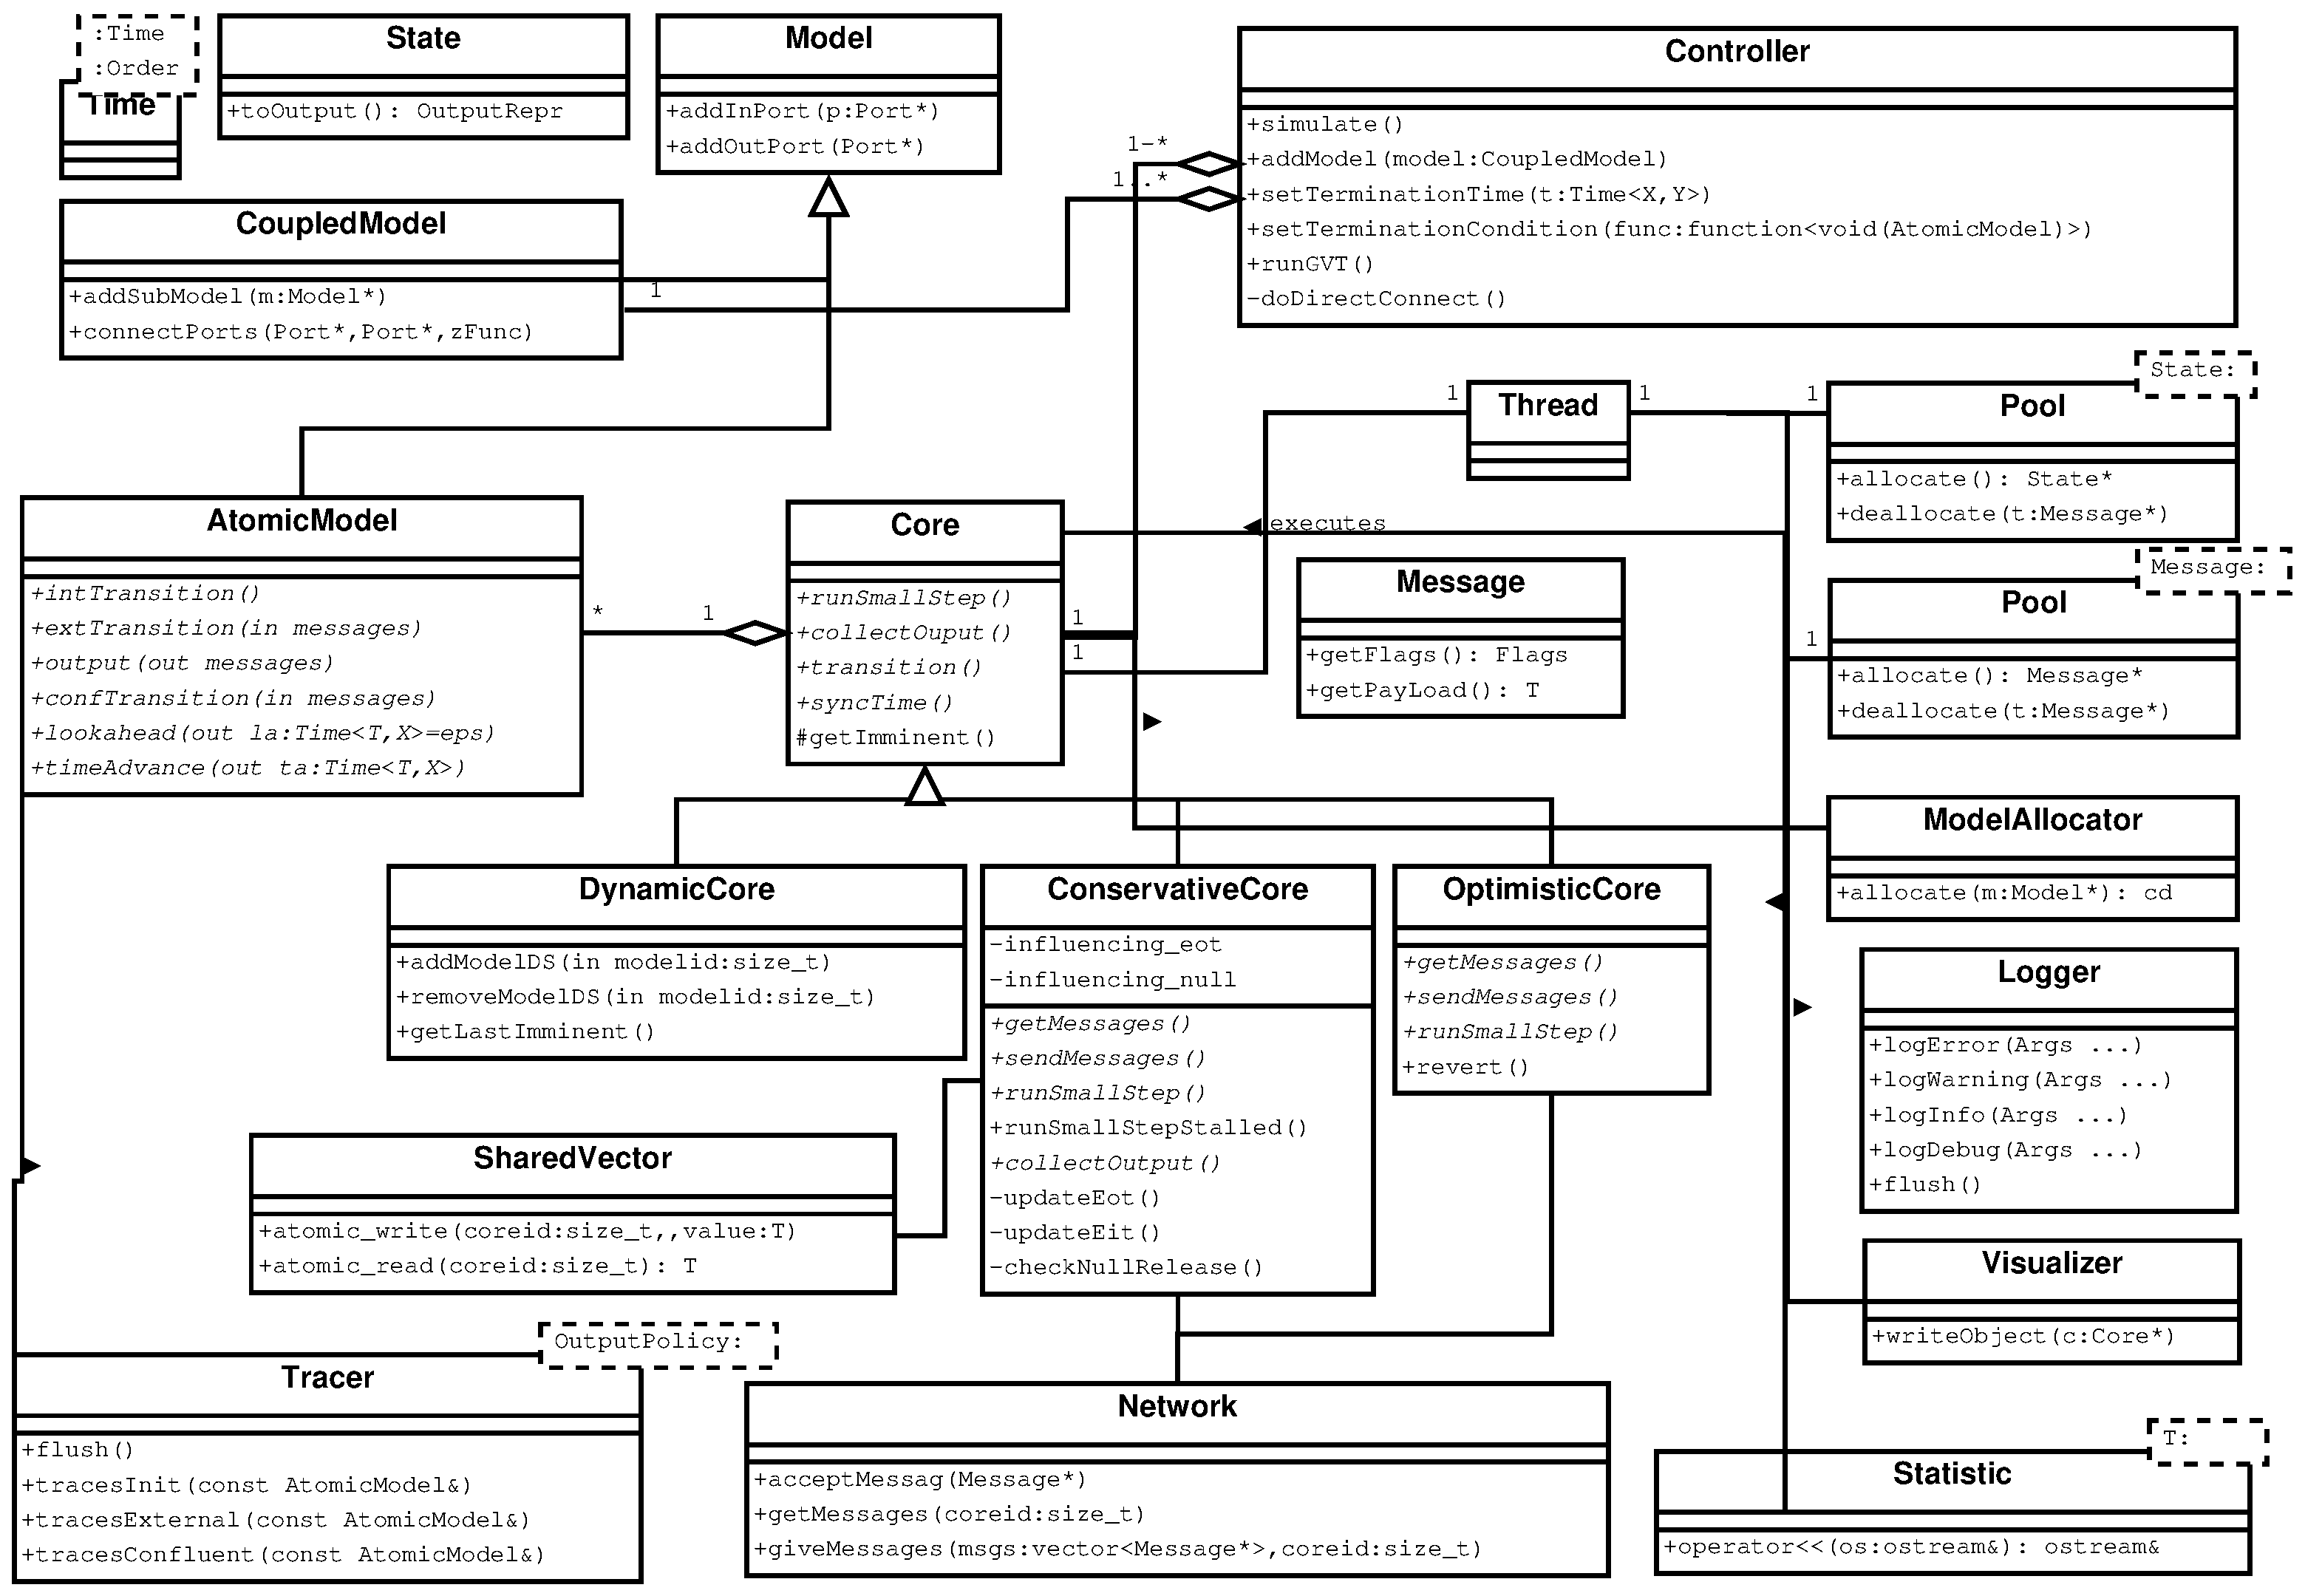
\includegraphics[width=\textwidth]{fig/cores_class_diagram.eps}
	\caption{Dxex design.}
	\label{fig:class_diagram}
\end{figure*}

\subsubsection{Conservative}
For conservative synchronization, each node must determine the nodes it is influenced by.
Each model needs to provide a lookahead function, which determines the lookahead depending on the current simulation state.
Within the returned time interval, the model promises not to raise an event.
A node aggregates this information to compute its earliest output time (EOT).
This value is written out in shared memory, where it can be read out by all other nodes.

Reading and writing to shared memory is done through the use of the new C++11 synchronization primitives.
Whereas this was also possible in previous versions of the C++ standard, by falling back to non-portable C functions, it was not a part of the C++ language standard.
C++11 further allows us to make the implementation portable, as well as more efficient: the compiler might know of optimizations specific to atomic variables or constant expressions which are heavily used in dxex.

\subsubsection{Optimistic}
For optimistic synchronization, each node must be able to roll back to a previous point in time.
This is often implemented through the use of state saving.
This needs to be done carefully in order to avoid unnecessary copies, and minimize the overhead.
We use the default: explicitly save each and every intermediate state.
Mattern's algorithm~\cite{mattern} is used to determine the GVT, as it runs asynchronously and uses only $2n$ synchronization messages.
Once the GVT is found, all nodes are informed of the new value, after which fossil collection is performed, and irreversible actions are committed.

The main problem we encountered in our implementation is the aggressive use of memory.
Frequent memory allocation and deallocation caused significant overheads, certainly when multiple threads do so concurrently.
This made us switch to the use of thread-local (using \textit{tcmalloc}) memory pools.
Again, we made use of specific new features of C++11, that were not available in Python, or even previous versions of the C++ language standard.

\subsection{Synchronization Protocol Transparency}
We define synchronization protocol transparency as having a single model, which always can be executed on each supported synchronization kernel, without any modifications.
User should thus only provide one model, implemented in C++11, which can be either using sequential execution, using conservative synchronization, or using optimistic synchronization.
Switching between simulation kernels is as simple as altering the simulation termination time.
The exception is conservative synchronization, where a lookahead function is required, which is not used in other synchronization kernels.
Two options are possible: either a lookahead function must always be provided, even when it is not required and possibly not used, or we use a default lookahead function if none is defined.

Always defining a lookahead function might seem redundant, especially if users will never use conservative synchronization.
Especially since defining the lookahead is often non-trivial and dependent on intricate model details.
The more attractive option is for the simulation tool to provide a default lookahead function, such that simulation can run anyway, but likely not at peak performance.
Depending on the model, simulation performance might still be faster than sequential simulation. 

Defining a lookahead function is therefore recommended in combination with conservative synchronization, but is not a necessity, as a default $epsilon$ (\textit{i.e.}, the smallest representable timestep) is used otherwise.

\subsection{Increasing Parallelism}
The goal of our contribution is to increase simulation performance as much as possible, leveraging parallel computation in the process.
Parallelizing the simulation kernel goes further, however, than merely implementing the different synchronization protocols.

We observed that after implementing all synchronization protocols, performance was still not within acceptable levels.
Profiling revealed that most of the overhead was caused by two issues: memory management and random number generation.
For both, it is already known that they can have significantly impact on parallelizability of code, since they introduce sequential blocks.
Both were tackled using approaches that are in common use in the parallel programming world.
We briefly mention how the application of these techniques influences our performance.

\subsubsection{Memory Management}
\label{sec:4-subsec:overhead-pgraph:memory}
\begin{figure}
    \center
    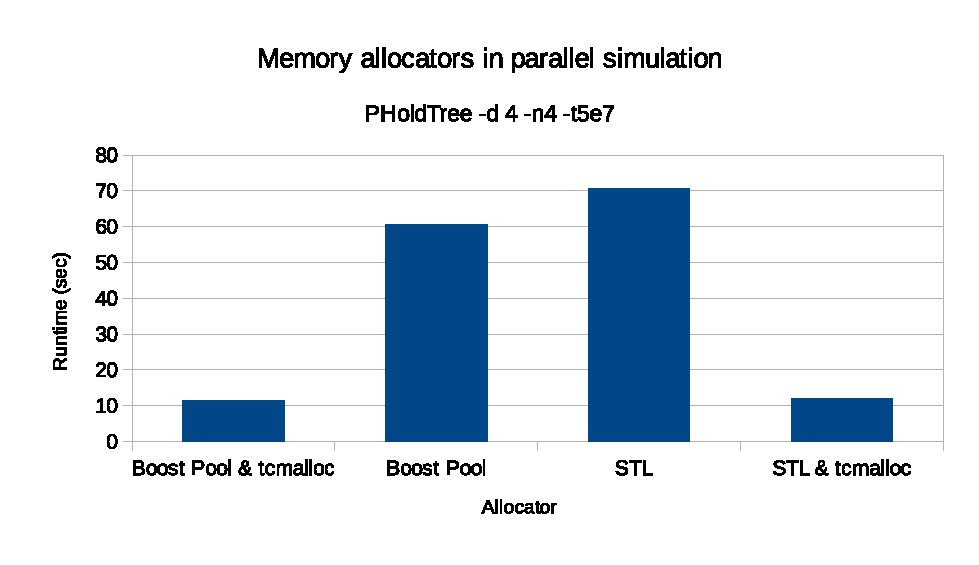
\includegraphics[width=\columnwidth]{fig/memory_allocators_parallel.eps}
    \caption{Effect of memory allocators on parallel execution time.}
    \label{fig:memallocators_parallel}
\end{figure}
Memory management is traditionally seen as one of the major bottlenecks in parallel computation~\cite{Memory}: memory bandwidth doesn't increase as fast as the number of cores using it.
While this is always a problem, it is aggravated in dxex by providing automatic memory management for events and states.
A model written for a sequential simulation will run correctly in a conservative or optimistic simulation without altering (from the point of view of the model author) the (de)allocation semantics of events or states.

Furthermore, allocating and deallocating memory by making calls to the operating system, as typically done by calls such as \texttt{malloc}, happens sequentially.
To counter this, our memory allocators are backed by a thread-aware pooling library.
In a sequential simulation kernel no allocated event will persist beyond a single time advance, even allowing the use of an arena-style allocator.
Conservative and optimistic simulation need to use generic pool allocators since events are shared across kernels and thus have a different lifetime.

%TODO what does it mean to "pool aggressively?"
Intra-kernel events are pooled aggressively, whereas inter-kernel events need a GVT algorithm to determine when safe deallocation can occur, even in conservative synchronization.
A simulation with many inter kernel events suffers a performance hit, whereas the impact of many intra kernel events can be minimized using arena allocators.

Dxex uses Boost Pool~\cite{boostpool} allocators in parallel simulation kernels and arena-style allocators for sequential simulation.
The latter can be faster, but at the cost of extra configuration.
The allocators are supplemented by the library \textit{tcmalloc}~\cite{tcmalloc}, which reduces lock contention in \texttt{malloc} calls.

We primarily investigate this for optimistic simulation, as this is the most memory consuming mode of simulation~\cite{Fujimoto}.
Simulation execution times for all four combinations are shown in Figure~\ref{fig:memallocators_parallel}.
Optimistic simulation greatly benefits from the use of \textit{tcmalloc}, regardless of the allocator.
Nonetheless the pool allocator also reduces the allocation overhead, though only by a relatively small fraction.
Both techniques are required to reduce the overhead of memory allocations in dxex, and on by default.

Both pools and \textit{tcmalloc} try to keep memory allocated instead of returning it to the Operating System (OS).
As a result, the OS will usually report memory consumption that is higher than the actual amount of stored data.

\subsubsection{Random Number Generators}
Random Number Generators (RNG) are another aspect of the program that results in sequentialization.
All accesses to the RNG will result in the modification of a global (\textit{i.e.}, shared between threads) variable.
This easily becomes a bottleneck in simulation, since random numbers are a common occurence in simulation~\cite{?}.
As such, a non-trivial amount of time in a simulation is often spent waiting for an RNG.

We of course still need to guarantee determinism and isolation between the calls to the RNG, as well as avoiding excessive synchronization.
Dxex uses the Tina RNG collection (TRNG)~\cite{PhysRevE.75.066701} as an alternative random number generator with performance and multithreading in mind.
Since the RNG is an implicit part of the state in the DEVS formalism, though often not implemented as such, we evaluated performance for both approaches: one global RNG per thread, and one RNG per atomic DEVS model.

We see in Figure~\ref{fig:Queuerngspeedup} that storing the RNG in the state is very expensive for the default STL random number generator.
%TODO fill in values
This is primarily caused by the significant difference in size: 2504 bytes for the STL random number generator, and 24 bytes for the Tina random number generator.
Dxex's sequential and conservative kernels are insensitive to storing the RNG object in the atomic model state, since no copying/state saving occurs in dxex conservative simulation.
The optimistic kernel is clearly affected, as it needs to copy more bytes in every transition due to state saving.

Figure~\ref{fig:Queuerngspeedup} shows that dxex in sequential simulation gets three times faster by using TRNG, than when using the STL RNG.
For parallel simulation, the synchronization overhead seems to be the main bottleneck, as seen by the big speedup gap between sequential and parallel simulation.
Conservative synchronization is almost insensitive to the changing of the RNG, though a slight increase in performance can be noted.
Optimistic synchronization gets much slower when the RNG becomes part of the model state, since the state needs to be copied as well.
This becomes a significant overhead when using the STL RNG, since performance plummets to a fraction of the original.
Using TRNG avoids this problem completely, as the size of the RNG state is negligible.

\begin{figure}
    \center
    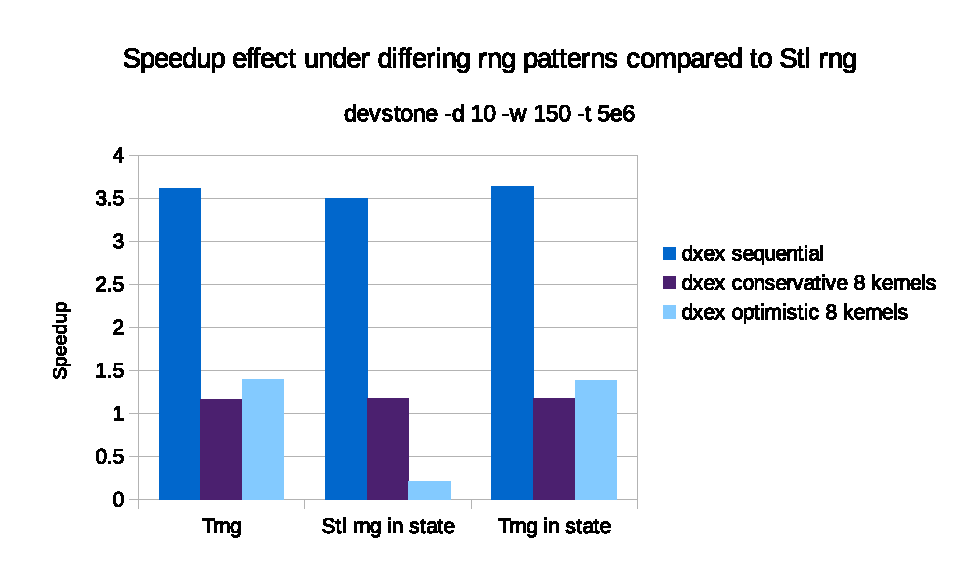
\includegraphics[width=\columnwidth]{fig/rngspeedupeffectdevstone.eps}
    \caption{Speedup with different RNG usage patterns compared to STL random number generator.}
    \label{fig:Queuerngspeedup}
\end{figure}


\section{Performance Evaluation}
\label{sec:4-performance}
In this section, we evaluate the performance of different synchronization protocols in \textit{dxex}.
We also compare to \textit{adevs}~\cite{adevs}, currently one of the most efficient simulation kernels~\cite{DEVStoneJournal,DEVSSurvey}, to show that our modularity does not impede performance.
CPU time and memory usage is compared for both single core and multi core simulation.

We start off with a comparison of single core simulation, to show how \textit{adevs} and \textit{dxex} relate in this simple case.
For the multi core simulation benchmarks, results are presented for both conservative and optimistic synchronization.
We conclude with a comparison between inter and intra kernel parallelization and give use cases where these protocols can complement each other in the context of recent theoretical work ~\cite{amdahlpdevs}. 

For all benchmarks, results are well within a 5\% deviation of the average, such that only the average is used in the remainder of this section.
The same compilation flags were used for both \textit{adevs} and \textit{dxex} benchmarks (``\texttt{-O3 -flto}'').
To guarantee comparable results, no I/O was performed during benchmarks.
Before benchmarking, simulation traces were used to verify that \textit{adevs} and \textit{dxex} return exactly the same simulation results.
Benchmarks were performed using Linux, but our simulation tool works equally well on Windows and Mac.
The exact parameters for each benchmark can be found in our repository. 

The benchmarks are ran on a machine with 8 x AMD Opteron(TM) Processor 6274 with 8 cores per CPU (for a total of 64 cores) and 192 GB RAM.

\subsection{Benchmark Models}
We use three different benchmark models, covering different aspects of the simulation kernel.

First, the \textit{Queue} model, based on the \textit{HI} model of DEVStone~\cite{DEVStone}, creates a chain of hierarchically nested atomic \textsf{DEVS} models.
A single generator pushes events into the queue, which get consumed by the processors after a fixed or random delay.
It takes two parameters: the width and depth of the hierarchy.
This benchmark shows how the complexity of the simulation kernel behaves for an increasing amount of atomic models, and an increasingly deep hierarchy.
An example for a width and depth of 2 is shown in Figure~\ref{fig:queue_model}.
	
Second, the \textit{Interconnect} model, a merge of PHOLD~\cite{PHOLD} and the \textit{HI} model of DEVStone~\cite{DEVStone}, creates $n$ atomic models, where each model has exactly one output port.
Similar to PHOLD, all models are connected to one another, but all through the same port: every model receives each generated event (\textit{i.e.}, the event is broadcasted).
The model takes one parameter: the number of models.
This benchmark shows the complexity of event creation, event routing, and simultaneous event handling.
An example for three models is shown in Figure~\ref{fig:interconnect_model}.

Third, the \textit{PHOLD} model~\cite{PHOLD}, creates $n$ atomic models, where each model has exactly $n-1$ output ports.
Each atomic model is directly connected to every other atomic model.
After a random delay, an atomic model sends out an event to a randomly selected output port.
Output port selection happens in two phases: first it is decided whether the event should be sent within the same node, or outside of the node.
Afterwards, a uniform selection is made between the remaining models.
The model takes two parameters: the percentage of remote events (determining the percentage of messages routed to other nodes), and the percentage of high-priority events.
High-priority events are events generated in a very short time after the previous event.
This benchmark shows how the simulation kernel behaves in the presence of many local or remote events, in combination with a varying percentage of high-priority events.
An example for four models, split over two nodes, is shown in Figure~\ref{fig:PHOLD_model}.

\begin{figure}
	\center
	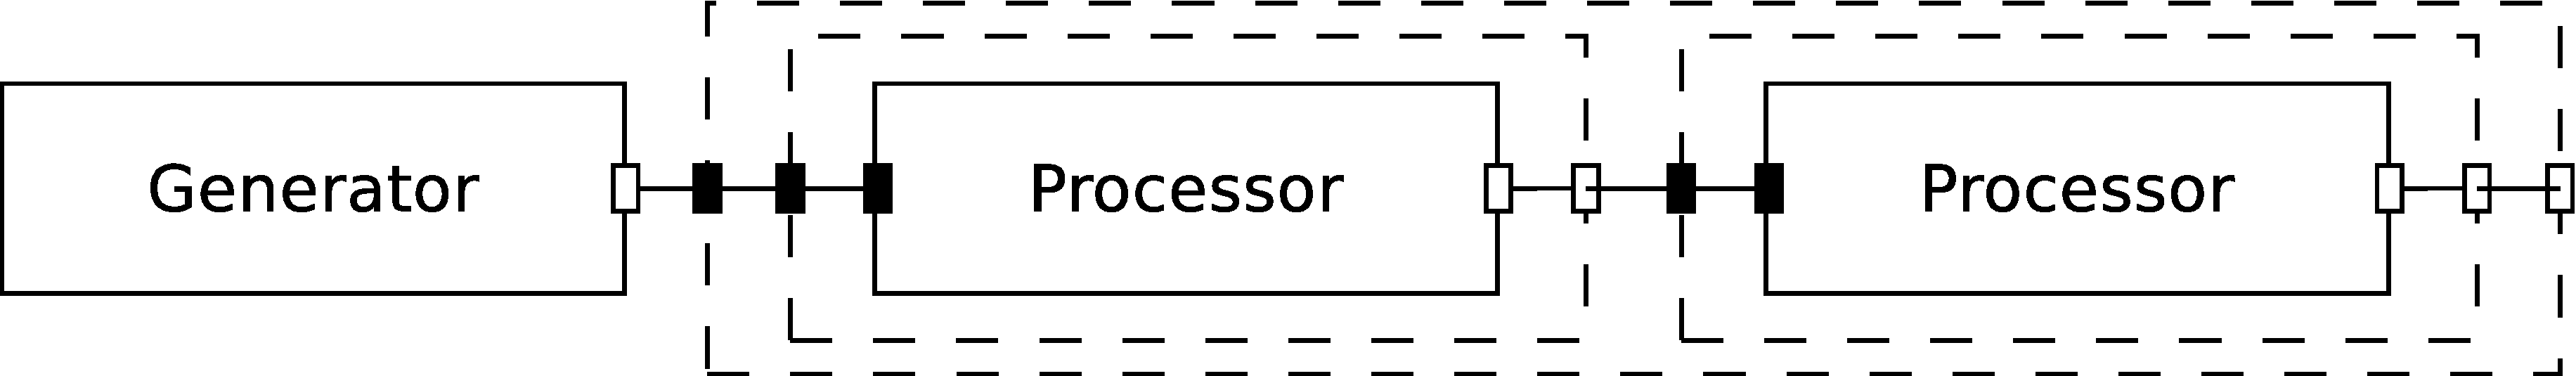
\includegraphics[width=\columnwidth]{fig/queue_model_fixed.pdf}
	\caption{Queue model for depth and width 2.}
	\label{fig:queue_model}
\end{figure}
	
\begin{figure}
    \center
	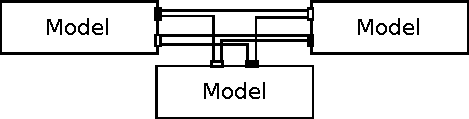
\includegraphics[width=\modelfraction\columnwidth]{fig/interconnect_model.pdf}
	\caption{Interconnect model for three models.}
	\label{fig:interconnect_model}
\end{figure}

\begin{figure}
    \center
	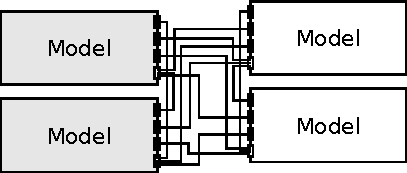
\includegraphics[width=\modelfraction\columnwidth]{fig/phold_model.pdf}
	\caption{PHOLD model for four models. Color denotes the two nodes.}
	\label{fig:PHOLD_model}
\end{figure}

\subsection{Single Core Simulation}
We start by evaluating single core simulation performance, in order to obtain a baseline for our comparison of multi core simulation performance.

\subsubsection{Queue}
\label{4-seq-Queue}
For the first benchmark, we tested the effect of hierarchical complexity of the model in the performance of the simulator.
A set of three tests was performed, where each test has the same number of models but an increasing depth.
The results can be seen in Figure~\ref{fig:Queue_benchmark_seq}.
Since \textit{dxex} performs direct connection~\cite{SymbolicFlattening} on the model, there is no performance hit when the depth is increased.
Direct connection only needs to be done at initialization, so it is a one time cost that is negligible for long running simulations.
\textit{Adevs}, on the other hand, suffers from the increased depth, even though some similar (but not identical) optimization to event passing was made~\cite{adevs_opt}.
With every new hierarchical layer, routing an event from one atomic model to the next becomes more expensive, resulting in an increase in runtime.

\begin{figure}
	\center
	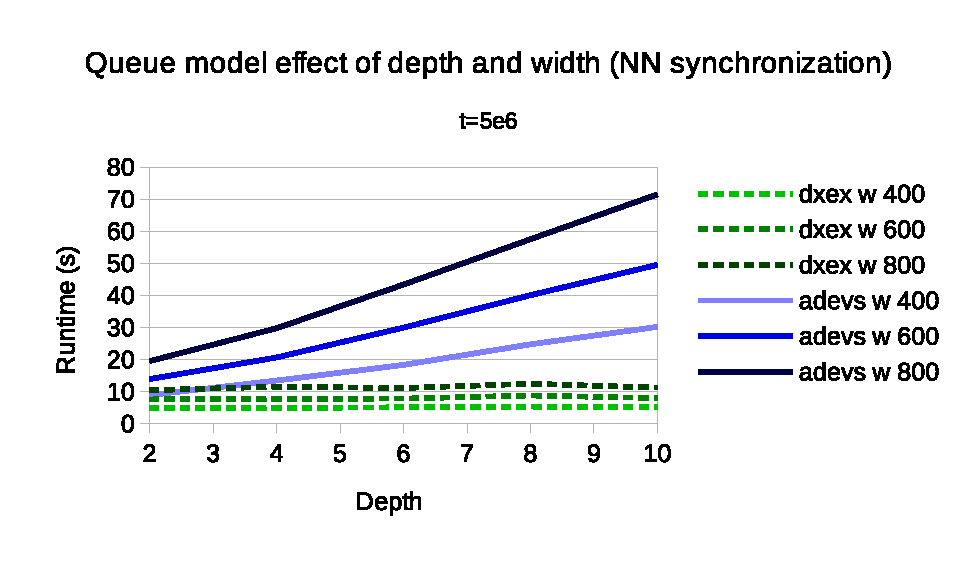
\includegraphics[width=\columnwidth]{fig/queue_fixed_sequential.eps}
	\caption{Queue benchmark results for single core simulation.}
	\label{fig:Queue_benchmark_seq}
\end{figure}

\subsubsection{Interconnect}
\label{4-seq-Interconnect}
In the Interconnect model, we increase the number of atomic models, quadratically increasing the number of couplings and the number of external transitions.
As shown in Figure~\ref{fig:Interconnect_benchmark}, \textit{adevs} now outperforms \textit{dxex} by a fair margin.
Analysis showed that this is caused by the high amount of events: event creation is much slower in \textit{dxex} than it is in \textit{adevs}, despite \textit{dxex}'s use of memory pools.
To shield the user from threading and deallocation concerns, \textit{dxex} provides an event superclass from which the user can derive to create a specialized event type.
Copying, deallocation, and tracing are done at runtime, adding significant overhead when events happen frequently.
Profiling the benchmarks revealed the increased cost of output generation and deallocation as the determining factor.

\begin{figure}
	\center
	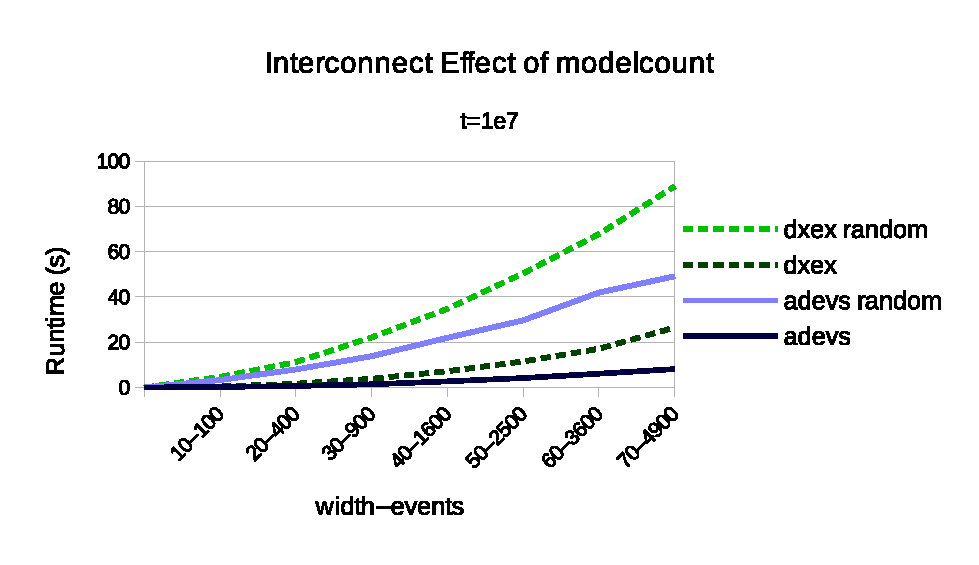
\includegraphics[width=\columnwidth]{fig/interconnect_sequential.eps}
	\caption{Interconnect benchmark results for single core simulation.}
	\label{fig:Interconnect_benchmark}
\end{figure}

\subsubsection{PHold}
\label{4-seq-PHold}
The PHold model is very similar to the Interconnect model.
The biggest difference is that the amount of messages sent is much lower.
The number of events scales linear with the number of models, not quadratic.
Figure~\ref{fig:Phold_benchmark} shows that in terms of performance \textit{dxex} and \textit{adevs} are very close to each other, with \textit{adevs} slightly outperforming \textit{dxex}.

\begin{figure}
	\center
	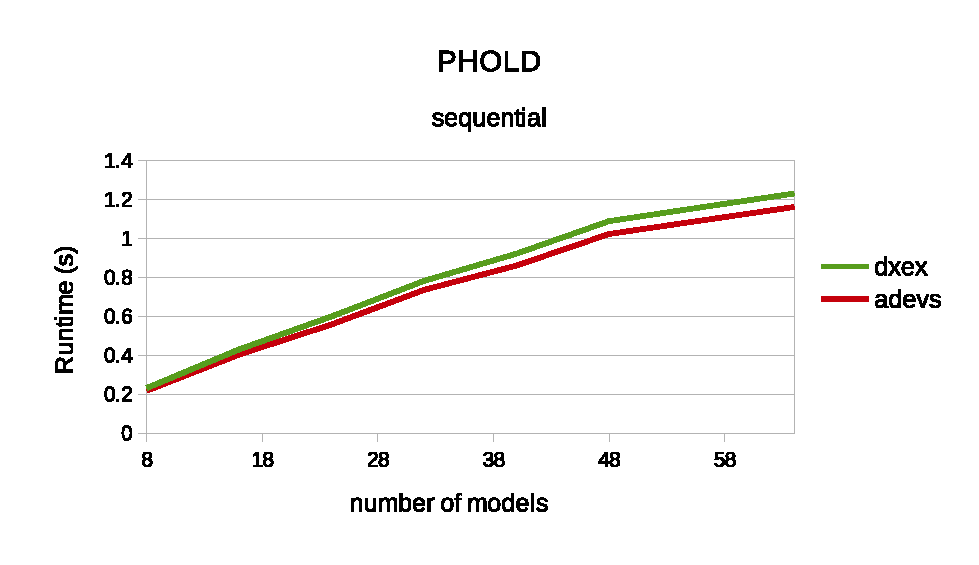
\includegraphics[width=\columnwidth]{fig/phold_sequential.eps}
	\caption{PHold benchmark results for single core simulation.}
	\label{fig:Phold_benchmark}
\end{figure}

\subsection{Parallel Simulation}
We now continue by describing our multi core simulation performance for different synchronization protocols, and compared to \textit{adevs}.
The speedup of \textit{adevs} is computed with the corresponding \textit{dxex} single core benchmark.
This was done to take into account the performance difference observed in single core simulation.
As such, the highest speedup indicates the fastest results among all tools, independent of single core simulation results.

\subsubsection{Queue}
The Queue model is one single chain of models, resembling a pipeline.
This structure can be exploited to prevent cyclic dependencies in the multi core simulation.

Figure~\ref{fig:Queue_plot_strong} shows the speedup compared to single core simulation for a fixed problem size (\textit{i.e.}, strong scaling).
As the number of kernels increases, the optimistic protocol quickly becomes the worst choice.
This is mainly caused by the pipeline structure of the model: the last models in the queue only respond to incoming messages and therefore have to be rolled back frequently.
The difference between \textit{dxex} conservative protocol and \textit{adevs} becomes smaller when more and more cores are used.
The same effect can be seen when the problem size is increased in tandem with the number of used cores (\textit{i.e.}, weak scaling) in Figure~\ref{fig:Queue_plot_weak}.

\begin{figure}
	\center
	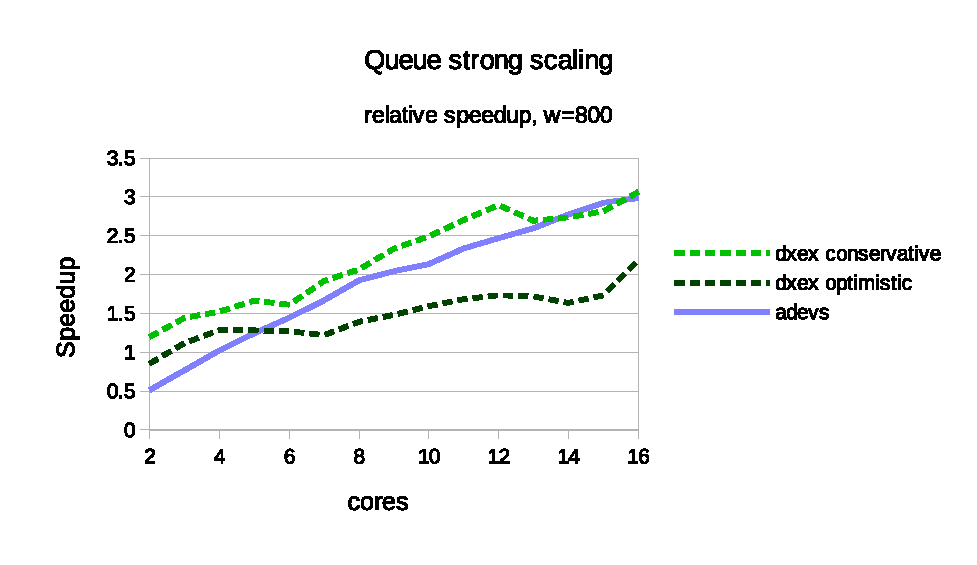
\includegraphics[width=\columnwidth]{fig/queue_fixed_strong_speedup.eps}
	\caption{Queue model strong scaling speedup compared to \textit{dxex} single core.}
	\label{fig:Queue_plot_strong}
\end{figure}

\begin{figure}
	\center
	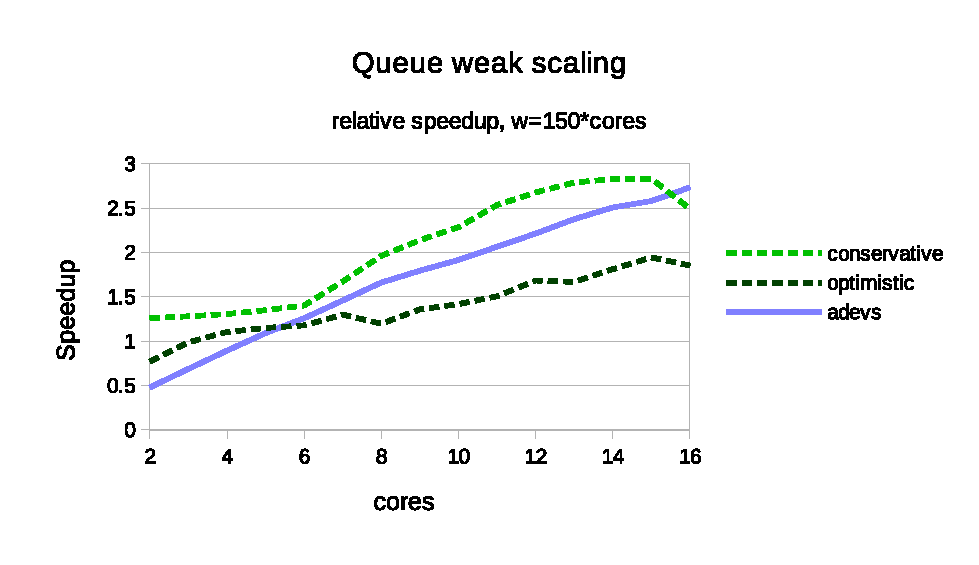
\includegraphics[width=\columnwidth]{fig/queue_fixed_weak_speedup.eps}
	\caption{Queue model weak scaling speedup compared to \textit{dxex} single core.}
	\label{fig:Queue_plot_weak}
\end{figure}
	
\subsubsection{Interconnect}
\label{subsec:parallelinterconnect}
In the Interconnect model, we determine how broadcast communication is supported across multiple nodes.
The number of models is now kept constant at eight.
Results are shown in Figure~\ref{fig:interconnect_benchmark_parallel}.
When the number of nodes increases, performance decreases due to increasing contention in conservative simulation and the increasing number of rollbacks in optimistic simulation.
All models depend on each other and have no computational load whatsoever, negating any possible performance gain by executing the simulation in a multi core setting.

\begin{figure}
	\center
	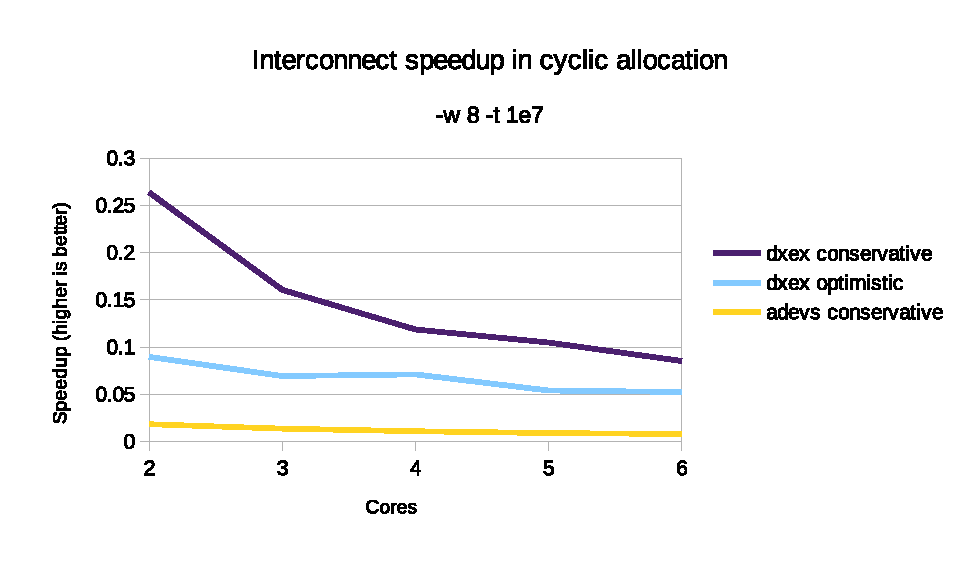
\includegraphics[width=\columnwidth]{fig/interconnect_parallel.eps}
    %TODO cyclic allocation in title?
	\caption{Interconnect benchmark results for multi core simulation.}
	\label{fig:interconnect_benchmark_parallel}
\end{figure}

\subsubsection{PHOLD}
In the PHOLD model, we first investigate the influence of the percentage of remote events on the speedup.
A remote event in this context is an event that is sent from a model on one kernel to a model on another simulation kernel.
When remote events are rare, optimistic synchronization rarely has to roll back, thus increasing performance.
With more frequent remote events, however, optimistic synchronization quickly slows down due to frequent rollbacks.
Conservative synchronization, on the other hand, is mostly unconcerned with the number of remote events: the mere fact that a remote event can happen, causes it to block and wait.
Even though a single synchronization protocol is always ideal in this case, it already shows that different synchronization protocols respond differently to a changing model.

\textit{Adevs} is significantly slower during conservative synchronization.
Analysis of profiling callgraphs shows that exception handling in \textit{adevs} is the main cause. 
To keep the models equivalent, the \textit{adevs} version does not provide the \{begin,end\}Lookahead methods, which accounts for the exception handling.
These functions require the user to implement a state saving method.
But in contrast to \textit{PythonPDEVS} and \textit{dxex}, which handle this inside the kernel, users need to manually define this.
We feel this would lead to an unfair comparison as we would like to keep the models agnostic of the underlying protocols across all benchmarks.

\begin{figure}
    \center
    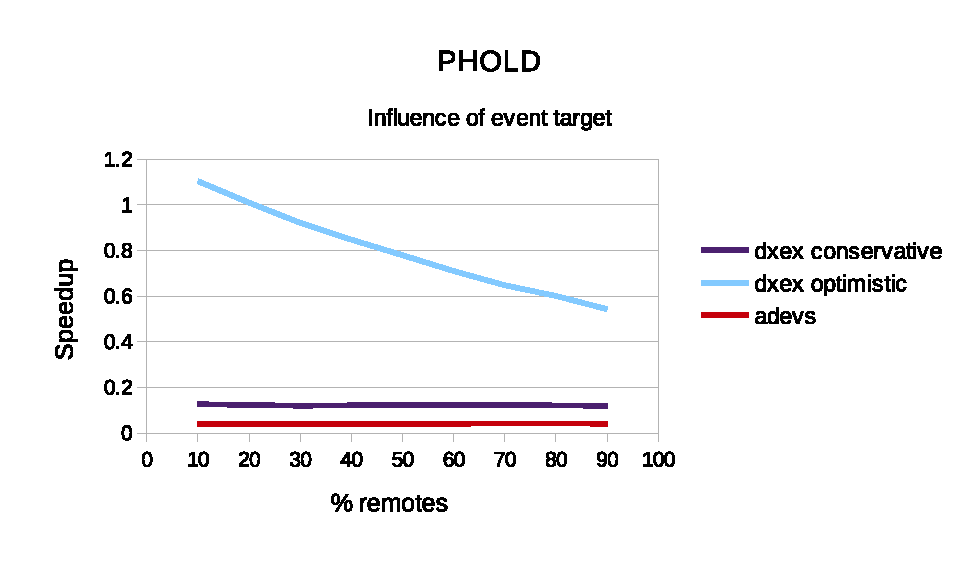
\includegraphics[width=\columnwidth]{fig/phold_remotes.eps}
    \caption{PHOLD benchmark results for multi core simulation using four kernels, with varying percentage of remote events.}
\end{figure}

\begin{figure}
	\center
	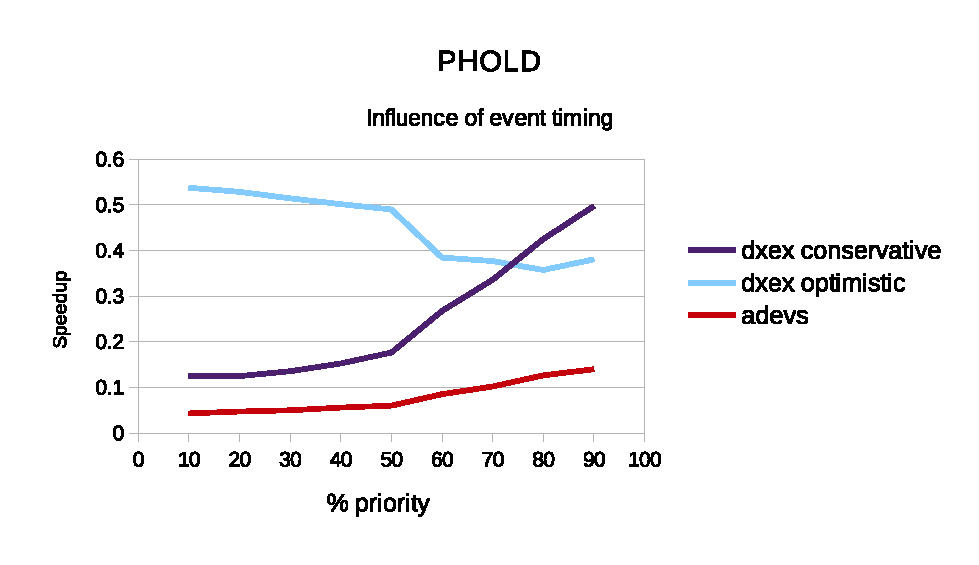
\includegraphics[width=\columnwidth]{fig/phold_priority.eps}
	\caption{PHOLD benchmark results for multi core simulation using four kernels, with varying amount of high-priority events.}
	\label{fig:phold_priority}
\end{figure}

Contrary to normal events, high-priority events happen almost instantaneously, restricting lookahead to a very small value.
Even when normal events occur most often, conservative synchronization always blocks until it can make guarantees.
Optimistic synchronization, however, simply goes forward in simulation time and rolls back when these high-priority events happen.
This situation closely mimics the model typically used for comparing conservative and optimistic synchronization~\cite{FujimotoBook}.

Figure~\ref{fig:phold_priority} shows how simulation performance is influenced by the fraction of these high-priority events.
If barely any high-priority events occur, conservative synchronization is penalized due to its excessive blocking, which often turned out to be unnecessary.
When many high-priority events occur, optimistic synchronization is penalized due to its unconditional progression of simulation, which frequently needs to be rolled back.
Results show that there is no single perfect synchronization algorithm for this kind of models: depending on configuration, either synchronization protocol might be better.

\subsection{Comparison to the abstract simulator}
The abstract simulator of \textsf{Parallel DEVS} included its own notion of parallelism: transition functions that happen at the same point in simulated time can be trivially parallelized. In this work we refer to this approach as \pSim so as not to confuse with the PDEVS formalism.
This parallelization is trivial, in the sense that there is no need for synchronization protocols.
The parallelization of the transition functions (from now on called the ``inherent parallelism'') is, at least in \textit{dxex}, independent of the use of a synchronization protocol.
That is, both can be used simultaneously.
Following the theoretical analysis published in~\cite{amdahlpdevs}, a comparison between this inherent parallelism and the use of synchronization protocols is warranted.

\paragraph{Model}
We have opted to use the \textit{Queue} model for this comparison, as it allows for many interesting configurations.
%TODO what is meant with this allocation of threads and synchronized kernels?
% 4 Kernels running on a dedicated thread, with per kernel 4 threads allocated to use for PDEVS.
The effect of combining 4 synchronized kernels, with each 4 threads for \pSim, is contrasted with 16 threads for \pSim and 16 kernels for conservative and optimistic.
The first scenario runs each kernel on a dedicated thread synchronized with the other 3 kernels. Each kernel can use up to 4 threads for \pSim. In the second scenario \pSim can use up to 16 threads while running in a single core kernel. Finally 16 synchronized kernels are used with one thread per kernel.
This allows us to observe which is more efficient in obtaining a speedup.
We simulate a computational load by an optional call to sleep in the transition functions set at 5 milliseconds.
The model is configured with depth 4 and width 300 if the transition function has no load, and width 50 if the computational load is active.
In our configuration, an imminent model always generates output, resulting in the receiving model becoming imminent.
The probability that an internal transition in a model generates output and is connected to a receiving model here is $1$. The probability that a model becomes immediately imminent depends on whether fixed or random timeadvance is used. In the case of fixed timeadvance, a model will always become immediately imminent. When random timeadvance is used, this probability is $\frac{1}{n}$, with $n$ denoting the total amount of atomic models. These probabilities correspond with the $q$ parameter in the theoretical analysis ~\cite{amdahlpdevs}. 
The probability that a model is imminent (i.e. is scheduled to execute an internal transition) at any given point in time in this model is equal to $1$ when a fixed timeadvance is used and $\frac{1}{n}$ when a random time advance is used. These probabilities correspond with the $p$ parameter in the theoretical analysis.

The benchmarks are run sufficiently long enough to guarantee that the frequency of internal and external transitions is equal within a benchmark, regardless of the randomness of the timeadvance. In our model each model will be executing internal and external transitions, creating an ideal use case to evaluate the speedup inherent parallelism can obtain. 
The key difference is that although the event frequency is the same, their concurrency is not. 
This benchmark combines both possible sources of parallelization : concurrent internal and external transitions. 
Models are equally distributed over the kernels and between threads in \pSim.
The coefficient of variation of our results is less than $1\%$.
The communication overhead is hard to estimate, but given our coefficient of variation, we can expect this overhead to be constant.

We consider two cases: one where all transition functions happen simultaneously, and one where transition functions never happen simultaneously.
We defer the discussion on which of these two is the most realistic, as this depends on the problem domain.
For example, in a simulation with a fixed timestep (\textit{e.g.}, cell-based models, discretization of continuous model), transition functions will often occur simultaneously.
Conversely, simulations with an arbitrary timestep (\textit{e.g.}, many independent systems communicating together) have very few simultaneous events.

\paragraph{Concurrent events}
First we create a model where all transitions happen simultaneously, with a significant computational load in the transition functions.
In Figure~\ref{fig:psim_plot_fixed_sleep}, we observe that exploiting only the inherent parallelism, results in a speedup of about 10.  
Simulation with conservative and optimistic synchronization is run first with 16 kernels, then with 4 kernels having 4 \pSim threads each. 
Both synchronization protocols achieve a speedup similar to only exploiting the inherent parallelism.
Combining the protocols with the inherent parallelism gives near identical results.
In this scenario there is no real advantage between the different parallel configurations.

\begin{figure}
	\center
	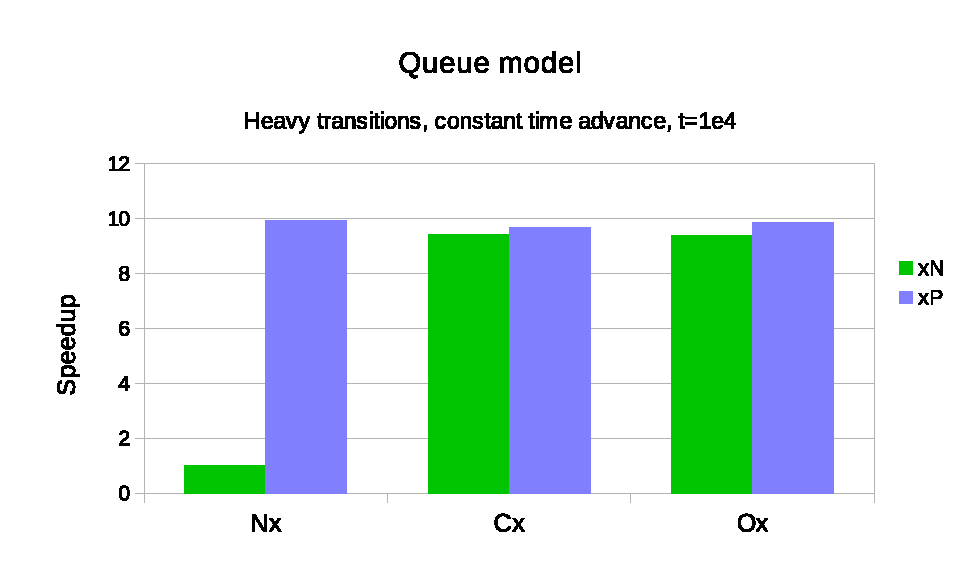
\includegraphics[width=\columnwidth]{fig/pdevs_fixed_sleep.eps}
	\caption{Queue speedup benchmark for PDEVS and synchronization with maximal concurrent events and significant computational load}
	\label{fig:psim_plot_fixed_sleep}
\end{figure}

\paragraph{Random events}
Now we randomize the time advance in the models, resulting in very few transition functions that happen simultaneously.
Even when two transitions are only minimally apart in simulated time, they cannot be executed in parallel, as there might otherwise be a causality error.
The transition function has the same computational load as in the previous configuration. 
The results in Figure~\ref{fig:psim_plot_random_sleep} show that parallelizing transition functions only, adds little overhead. 
Nonetheless, performance is not increased at all: the chances of executing a few transition functions in parallel does not make up for the overhead of checking.
In combination with either synchronization protocol, a minor improvement can still be seen, but this is primarily caused by the synchronization protocol, and not by parallelizing the transition functions.

\begin{figure}
	\center
	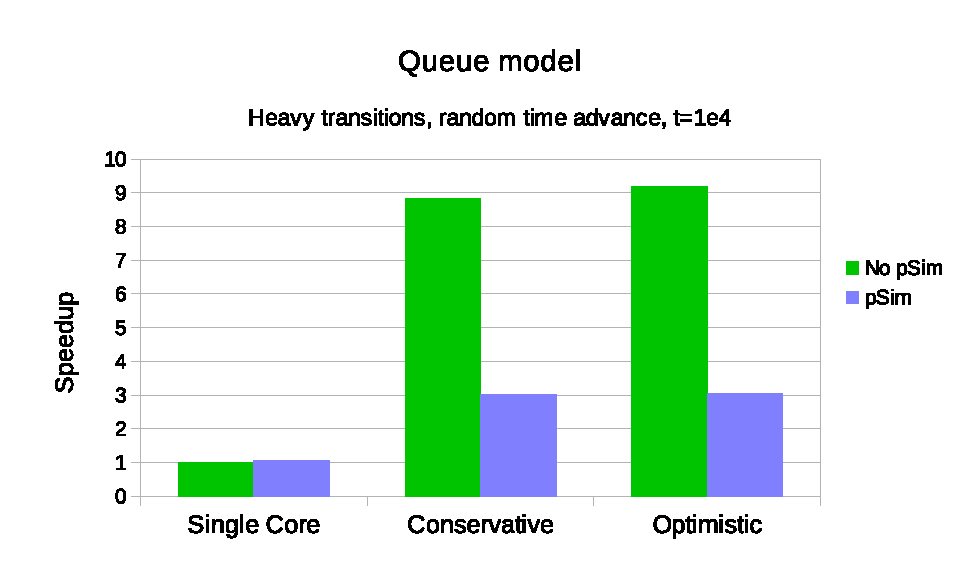
\includegraphics[width=\columnwidth]{fig/pdevs_random_sleep.eps}
	\caption{Queue speedup benchmark for PDEVS and synchronization with randomized events and significant computational load}
	\label{fig:psim_plot_random_sleep}
\end{figure}

\paragraph{Computational load}
Finally, we remove the computation load from the transition function, in combination with many concurrent events.
Figure~\ref{fig:psim_plot_no_sleep} shows that in single core simulation, the overhead of thread management and shared memory communication is crippling for performance.
Even though many events occur concurrently, the actual computation being done in the transition function does not outweigh the overhead, resulting in much slower simulation than single core execution of transition functions.
When combined with synchronization protocols, performance is still reasonable, though the use of the inherent parallelism is not beneficial either way.
Both synchronization protocols achieve a reasonable speedup without \pSim, as the overhead of thread management (creation and destruction) is avoided.
These results are similar to~\cite{Himmelspach}.
 
\begin{figure}
	\center
	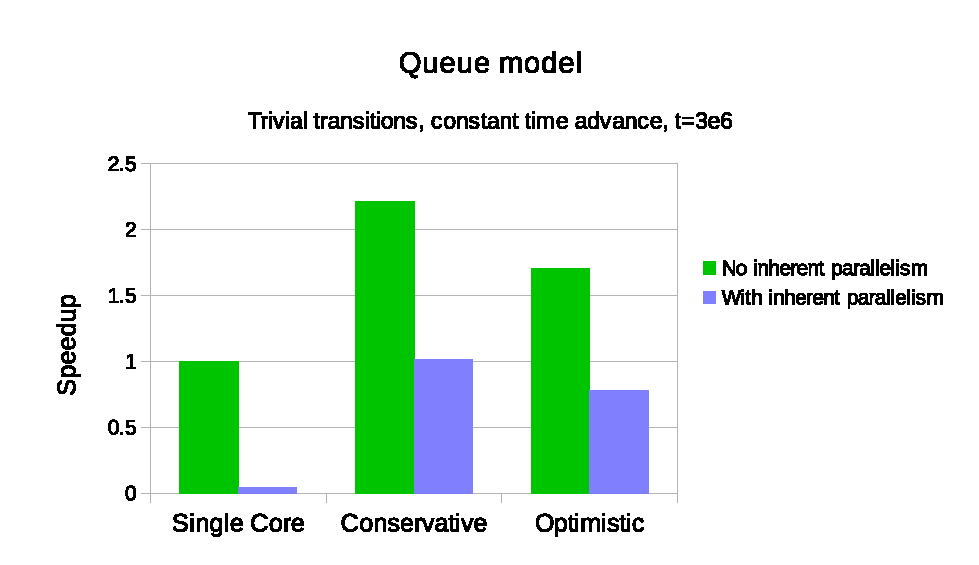
\includegraphics[width=\columnwidth]{fig/pdevs_no_sleep.eps}
	\caption{Queue speedup benchmark for PDEVS and synchronization with maximal concurrent events and trivial computational load}
	\label{fig:psim_plot_no_sleep}
\end{figure}

\paragraph{Discussion}
In \textit{dxex}, use of the inherent parallelism found in \textsf{Parallel DEVS} can be combined with any of the supported synchronization protocols.
The user is not forced to choose between either: the capabilities of the computer can be divided over both approaches.
While exploitation of the inherent parallelism can offer a significant speedup, a high number of transitions must be triggered simultaneously throughout the whole simulation.
Additionally, the computational load of the transition functions should be high enough to warrant the thread management overhead.
We conclude that both approaches have their distinct advantages and disadvantages.
The inherent parallelism of \textsf{Parallel DEVS} avoids synchronization overhead and is trivial to implement.
It is not influenced by the coupling of models, only by the number of simultaneous transition functions and the computational load in the transition function.
In contrast, either of the two synchronization protocols is heavily influenced by the coupling of the models, but not by the computational load or number of simultaneous transitions.

\subsection{Memory Usage}
Apart from simulation execution time, memory usage during simulation is also of great importance. Having insufficient memory may cause sudden deterioration in performance, even to the point of making the simulation infeasible.
We therefore also investigate the memory usage of different synchronization protocols, and again compare to \textit{adevs}.

We do not tackle the problem of states that become too large for a single machine to hold.
This problem can be mitigated by distribution over multiple machines, which neither \textit{dxex} nor \textit{adevs} support.

\subsubsection{Remarks}
Both \textit{dxex} and \textit{adevs} use \textit{tcmalloc} as memory allocator, allowing for thread-local allocation.
Additionally, dxex uses memory pools to further reduce the frequency of expensive system calls (\textit{e.g.}, malloc and free).
\textit{tcmalloc} only gradually releases memory back to the OS, whereas our pools will not do so at all.
Due to our motivation for memory usage analysis, we will only measure peak allocation in maximum resident set size as reported by the OS.

\subsubsection{Results}
Figure~\ref{fig:memory} shows the memory used by the different benchmarks.
Results are in megabytes, and show the total memory footprint of the running application (\textit{i.e.}, text, stack, and heap).
Note the logarithmic scale due to the high memory consumption of optimistic synchronization.

Unsurprisingly, optimistic synchronization results show very high memory usage due to the saved states.
Note the logarithmic scale that was used for this reason.
Optimistic synchronization results vary heavily depending on thread scheduling by the operating system, as this influences the drift between nodes. 
Comparing similar approaches, we notice that \textit{dxex} and \textit{adevs} have very similar memory use.

Conservative simulation always uses more memory than single core simulation, as is to be expected.
Additional memory is required for the multiple threads, but also to store all events that are processed simultaneously.

\begin{figure}
    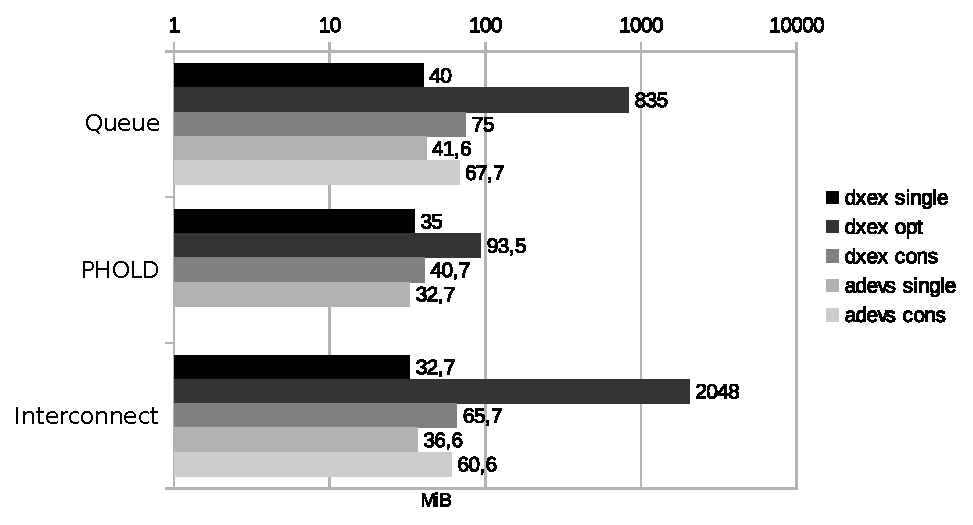
\includegraphics[width=\columnwidth]{fig/memory_voorlopig.eps}
    \caption{Memory usage results.}
    \label{fig:memory}
\end{figure}

\subsection{Conclusions on Performance Evaluation}
We have shown that our contribution is invaluable for high performance simulation: depending on the expected behaviour, modellers can choose the most appropriate synchronization protocol.
The use of synchronization protocols does also not prevent the exploitation of the inherent parallelism found in \textsf{ParallelPDEVS}.
Both approaches are useful in specific model configurations.
But even with the right synchronization protocol, we have seen that two problems remain.

First, although one of both synchronization protocols might be ideally suited for specific model behaviour, nothing guarantees that the model will exhibit the same behaviour throughout the simulation.
Similarly to the polymorphic scheduler~\cite{MasterThesis}, we wish to make it possible for the ideal option to be switched during simulation.
When changes to the model behaviour are noticed, the used synchronization protocol can be switched as well. 

Second, the allocation of models is nontrivial and has a significant impact on performance.
While our multi core speedup for the Queue model, for example, was rather high, this is mostly due to characteristics of the model: the dependency graph does not contain any cycles.
When cycles were introduced, as in the Interconnect model, performance became disastrous.

In the next two sections, we elaborate on these two problems.


\section{Runtime Switching}
\label{sec:4b-hotswap}
%TODO explain hotswapping
%TODO why hotswapping
Simply because a synchronization protocol is ideal at the start of the simulation, does not mean that it will still be ideal during the simulation.
It has been frequently shown, and repeated in the previous section, that model behaviour significantly influences the ideal synchronization protocol.
Contrary to many modelling formalisms, the DEVS formalisms makes it possible to model basically any kind of discrete event model.
As such, it is possible for the model to significantly change its behaviour throughout the simulation.

Defining the ideal synchronization protocol at the start of the simulation, when information about future model behaviour might be scarce, might therefore not offer the best possible performance.
In dxex, we not only make it possible to define the synchronization protocol to use, but also to change this decision throughout simulation.
To do this, all kernels are notified of the switch and they are forced to stop simulation using the current synchronization core.
When stopped, each kernel instantiates a new core that is provided with the simulation state of the previous core.
Simulation is then resumed with the new cores after the previous ones are destroyed.

As usual, switching imposes an overhead and should thus only be done if the benefits outweigh the induced overhead.
This overhead depends on the size of the model and the number of simulation cores.
For a simple model and a few cores, the overhead is less than a single second.

Although we currently only support manual switches between different synchronization protocols, this is not necessarily the case.
Ideally, a new component is added to the simulation kernel, which monitors model behaviour and simulation performance, and toggles between them automatically.
Our interface is thus augmented with the necessary bindings for such a component to be defined.
Also, our interface is augmented with an interface for statistics gathering and model behaviour analysis.
The implementation of such a component is currently left open: algorithms can be heavily based on machine learning or similar approaches.

\subsection{Statistics Gathering}
Traditionally, models are not exposed to simulation kernel details due to the wrong level of abstraction.
Simulation models only care about being simulated, and not about how this is being done.
This is different for a new simulation kernel component that has to monitor the behaviour of not only the model, but the simulator as well.

We add performance metrics in the simulation kernel, which logs relevant performance metrics and processes them for use in other components.
These metrics include the number of events created and destroyed, the number of inter and intra kernel events, the number of rollbacks, the measured lookahead, details of the Global Virtual Time (GVT) and Earliest Output Time (EOT) calculations, and basic information on the fairness between different simulation kernels.
With all these metrics, a component can get a fair view on both model and simulation kernel behaviour.

For example, if the actually seen lookahead is significantly higher than the defined lookahead, it might be interesting to switch to optimistic synchronization.
When the number of rollbacks is very high, conservative synchronization might be ideal.
And when neither of these two is an option, the simulation might just (temporarily) have to fall back to sequential simulation.

For performance reasons, statistics gathering is optional due to the imposed overhead.

\subsubsection{Visualization of Communication}
To provide some more insight in the models we used as benchmarks previously, we created a simple visualization of the simulation trace.
This trace visualizes the allocation of the model and all defined connections.
For each connection, the number of events transferred is annotated.
Examples are shown for the three benchmark models used before: Figures~\ref{fig:Queue_allocation},~\ref{fig:interconnect_allocation_parallel}, and~\ref{fig:phold_allocation} shows traces for the Queue, Interconnect, and PHOLD models respectively.

\begin{figure*}
    \center
    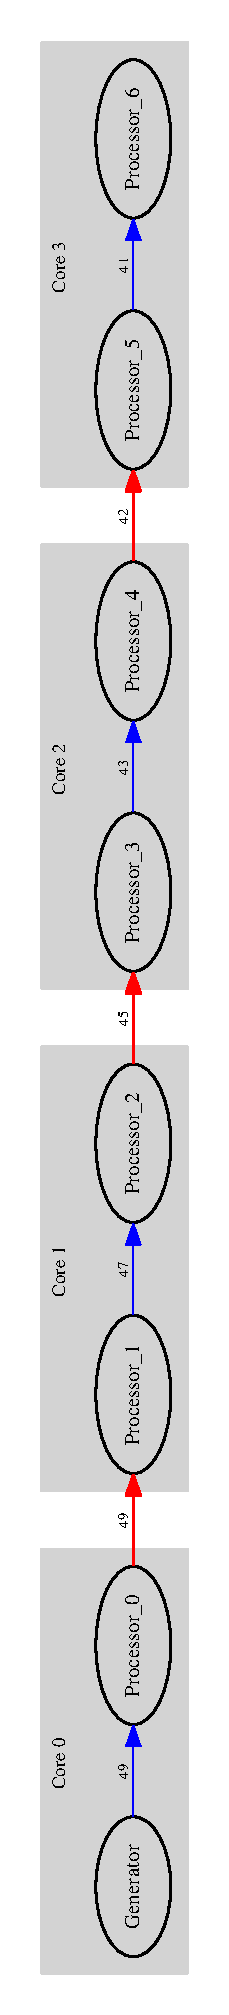
\includegraphics[height=\textwidth, angle=-90 ]{fig/queue_allocation.eps}
    \caption{Queue model simulation trace across 4 kernels.}
    \label{fig:Queue_allocation}
\end{figure*}
\begin{figure}
    \center
    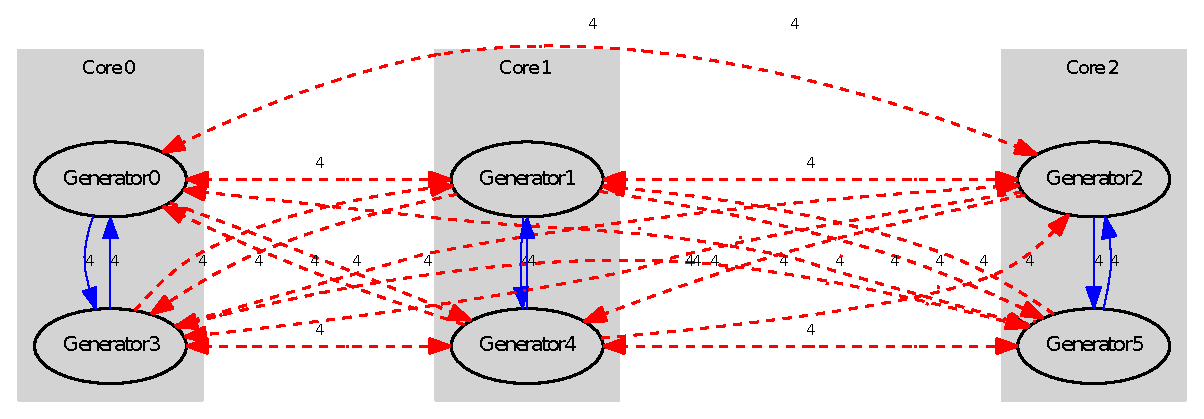
\includegraphics[width=\plotfraction\columnwidth]{fig/interconnect_parallel_allocation.eps}
    \caption{Interconnect simulation trace for 6 models on 3 kernels.}
    \label{fig:interconnect_allocation_parallel}
\end{figure}
\begin{figure}
    \center
    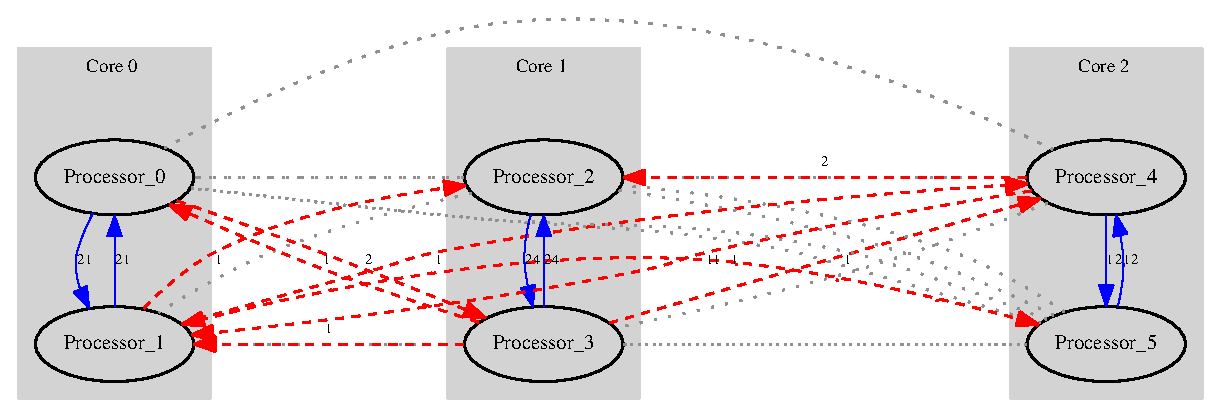
\includegraphics[width=\plotfraction\columnwidth]{fig/phold_parallel_allocation.eps}
    \caption{Phold simulation trace for parallel simulation using three kernels.}
    \label{fig:phold_allocation}
\end{figure}

Naturally, results similar to this are relevant information that can be used by the hotswapping component.


\section{Model Allocation}
\label{sec:4a-allocation}
\section{Model Allocation}
%TODO explain model allocation
%TODO why model allocation

\subsection{Performance Evaluation}
%TODO do basic performance evaluation of allocation
%TODO show model in statistics view

\subsection{Linking Back}
%TODO link back to initial performance evaluation

uthor can specify which kernel a model should be allocated to, should such manual intervention be required. This is handled by the default model allocator. If no preference is given a simple striping scheme is followed but this is not sufficient in most simulations to achieve a speedup in parallel. In Section \nameref{sec:4-performance} we analyse the performance impact of allocation schemes. By overriding the default allocator a model author can tune the allocation scheme for a specific model to maximize parallel speedup. This interface can be in future work also be used to employ graph algorithms for an automatic allocation scheme, for example one that avoids cycles in the resulting kernel dependency graph.


\section{Related Work}
\label{sec:5-related-work}
%TODO explain about other DEVS simulation kernels, and how they differ
%TODO explain about PythonPDEVS, the most related in terms of feature and "legacy" --> now in C++11 and way better performance
\subsection{PythonPDEVS}
Dxexmachina is closely related to PythonPDEVS in design and philosophy. PythonPDEVS allows anyone who grasps the DEVS formalisms to immediately simulate his/her model without having to consider the kernel implementation. C++ implementations cannot hope to match the fast prototype/edit/run cycles provided by PythonPDEVS, although this can be minimized by building the kernels as libraries. %maybe warn that if a header is touched, you still have to compile from scratch ? (eg. TIME_FP)
Advanced features such as activity based relocation and the performance gains this results in, are still unique to PythonPDEVS.
\subsection{Adevs}
%TODO explain about adevs, the most related in terms of performance --> we implement more synchronization options and offer better performance because ...
Adevs's source code is still under active development, allowing for an exact comparison in performance and features. It remains in most aspects the fastest simulation engine for the DEVS formalism, but it lacks an optimistic synchronization implementation. %Tracing ?
By virtue of not flattening Coupled Models, performance suffers in increasingly hierarchical models.
%checkme
\subsection{CD++}
%TODO explain about CD++, the most related in terms of synchronization --> we implement everything in a single program, with a non-fragmented code-base
%TODO make mention of Warped, which is the kernel used in CD++, and why we don't use it
Different projects on CD++ offer conservative (CCD++) as well as optimistic (PCD++) parallel simulation. In contrast to our single program, with a non-fragmented code-base, neither projects offer both synchronization protocols. CD++ relies on the WARPED kernel. It is a middleware that provides memory, event, file, time and communication scheduling. WARPED is not used here since we operate explicitly on a shared memory system and since we wanted to design our kernels using the least amount of overhead possible.


\section{Conclusions and Future Work}
\label{sec:6-conclusion}
%TODO conclude the paper, saying that our new simulation tool offers conservative and optimistic synchronization, resulting in good performance, which is even better than adevs
Sequentially dxex outperforms adevs in hierarchical simulations while yielding to adevs in broadcast-like simulations. 
Parallel the results are more nuanced. The sensitivity to broadcast simulations is carried over in the parallel implementation, resulting in performance loss for both synchronization protocols. Optimistic can still achieve good performance if the volume of inter-kernel messages is low. Both  are fast in non-cyclic simulations, with conservative better suited whenever state-saving becomes expensive and optimistic when lookahead is not available.\\
Finally, the current optimistic implementation is ill-suited for memory constrained systems, especially in simulations where the frequency of reverts is high.
\subsection{Future work}
%TODO future work: more things that we might want to implement, and probably something about automatically switching between synchronization protocols at runtime (and reference my activity papers ;))
\subsubsection{Memory}
Our optimistic implementation can benefit from a faster GVT algorithm such as FujiMoto's \cite{Fujimoto:1997:CGV:268403.268404}  or more recently \cite{Bauer:2005:SND:1069810.1070159}. 
With access to the memory subsystem in place (pools), optimistic could be constrained using per kernel quota preventing the simulation from exhausting memory. While less sensitive to memory pressure, the same approach could benefit conservative.
\subsubsection{Activity}
As shown in \cite{PythonPDEVS_ACTIMS} activity and allocation of models across kernels is a key aspect in achieving high performance in any parallel implementation. Allocating models so that there are no dependency cycles between their containing kernels is a first step, but not always possible. For optimistic one can use re-allocation to break (runtime dependency) cycles and/or perform load-balancing. If kernels are unevenly balanced they will begin to drift fast, causing increasingly more reverts. There is a limited framework implemented to track model activity for debugging purposes, this could be extended to enable the above strategies.
\subsubsection{Hybrid}
The optimistic implementation could use (null/eot/eit) from conservative to detect and/or reduce the cost of reverts without completely stalling on influencing kernels.
Conservative kernels could be extended with runtime information about influencing models, for example if one can guarantee a static dependency is not used for a fixed time-span, this can be removed for that period of (virtual) time. 
Ultimately the simulation could switch at runtime between protocols based on the information provided by activity tracking. This requires the above mentioned framework, and could only be done at timepoints where a GVT/LBTS time is agreed upon between the kernels. From the model point of view no changes are needed, although a non-trivial lookahead is obviously desired. 


\section*{ACKNOWLEDGMENTS}
This work was partly funded with a PhD fellowship grant from the Research Foundation - Flanders (FWO). 

\bibliographystyle{SageV}
\bibliography{papers}

\end{document}
